\documentclass[9pt,a4paper,]{extarticle}

\usepackage{f1000_styles}

\usepackage[pdfborder={0 0 0}]{hyperref}

\usepackage[numbers]{natbib}


%% maxwidth is the original width if it is less than linewidth
%% otherwise use linewidth (to make sure the graphics do not exceed the margin)
\makeatletter
\def\maxwidth{ %
  \ifdim\Gin@nat@width>\linewidth
    \linewidth
  \else
    \Gin@nat@width
  \fi
}
\makeatother

\usepackage{color}
\usepackage{fancyvrb}
\newcommand{\VerbBar}{|}
\newcommand{\VERB}{\Verb[commandchars=\\\{\}]}
\DefineVerbatimEnvironment{Highlighting}{Verbatim}{commandchars=\\\{\}}
% Add ',fontsize=\small' for more characters per line
\usepackage{framed}
\definecolor{shadecolor}{RGB}{248,248,248}
\newenvironment{Shaded}{\begin{snugshade}}{\end{snugshade}}
\newcommand{\KeywordTok}[1]{\textcolor[rgb]{0.13,0.29,0.53}{\textbf{#1}}}
\newcommand{\DataTypeTok}[1]{\textcolor[rgb]{0.13,0.29,0.53}{#1}}
\newcommand{\DecValTok}[1]{\textcolor[rgb]{0.00,0.00,0.81}{#1}}
\newcommand{\BaseNTok}[1]{\textcolor[rgb]{0.00,0.00,0.81}{#1}}
\newcommand{\FloatTok}[1]{\textcolor[rgb]{0.00,0.00,0.81}{#1}}
\newcommand{\ConstantTok}[1]{\textcolor[rgb]{0.00,0.00,0.00}{#1}}
\newcommand{\CharTok}[1]{\textcolor[rgb]{0.31,0.60,0.02}{#1}}
\newcommand{\SpecialCharTok}[1]{\textcolor[rgb]{0.00,0.00,0.00}{#1}}
\newcommand{\StringTok}[1]{\textcolor[rgb]{0.31,0.60,0.02}{#1}}
\newcommand{\VerbatimStringTok}[1]{\textcolor[rgb]{0.31,0.60,0.02}{#1}}
\newcommand{\SpecialStringTok}[1]{\textcolor[rgb]{0.31,0.60,0.02}{#1}}
\newcommand{\ImportTok}[1]{#1}
\newcommand{\CommentTok}[1]{\textcolor[rgb]{0.56,0.35,0.01}{\textit{#1}}}
\newcommand{\DocumentationTok}[1]{\textcolor[rgb]{0.56,0.35,0.01}{\textbf{\textit{#1}}}}
\newcommand{\AnnotationTok}[1]{\textcolor[rgb]{0.56,0.35,0.01}{\textbf{\textit{#1}}}}
\newcommand{\CommentVarTok}[1]{\textcolor[rgb]{0.56,0.35,0.01}{\textbf{\textit{#1}}}}
\newcommand{\OtherTok}[1]{\textcolor[rgb]{0.56,0.35,0.01}{#1}}
\newcommand{\FunctionTok}[1]{\textcolor[rgb]{0.00,0.00,0.00}{#1}}
\newcommand{\VariableTok}[1]{\textcolor[rgb]{0.00,0.00,0.00}{#1}}
\newcommand{\ControlFlowTok}[1]{\textcolor[rgb]{0.13,0.29,0.53}{\textbf{#1}}}
\newcommand{\OperatorTok}[1]{\textcolor[rgb]{0.81,0.36,0.00}{\textbf{#1}}}
\newcommand{\BuiltInTok}[1]{#1}
\newcommand{\ExtensionTok}[1]{#1}
\newcommand{\PreprocessorTok}[1]{\textcolor[rgb]{0.56,0.35,0.01}{\textit{#1}}}
\newcommand{\AttributeTok}[1]{\textcolor[rgb]{0.77,0.63,0.00}{#1}}
\newcommand{\RegionMarkerTok}[1]{#1}
\newcommand{\InformationTok}[1]{\textcolor[rgb]{0.56,0.35,0.01}{\textbf{\textit{#1}}}}
\newcommand{\WarningTok}[1]{\textcolor[rgb]{0.56,0.35,0.01}{\textbf{\textit{#1}}}}
\newcommand{\AlertTok}[1]{\textcolor[rgb]{0.94,0.16,0.16}{#1}}
\newcommand{\ErrorTok}[1]{\textcolor[rgb]{0.64,0.00,0.00}{\textbf{#1}}}
\newcommand{\NormalTok}[1]{#1}

% disable code chunks background
%\renewenvironment{Shaded}{}{}

% disable section numbers
\setcounter{secnumdepth}{0}


\usepackage{amsthm}
\newtheorem{theorem}{Theorem}
\newtheorem{lemma}{Lemma}
\theoremstyle{definition}
\newtheorem{definition}{Definition}
\newtheorem{corollary}{Corollary}
\newtheorem{proposition}{Proposition}
\theoremstyle{definition}
\newtheorem{example}{Example}
\theoremstyle{definition}
\newtheorem{exercise}{Exercise}
\theoremstyle{remark}
\newtheorem*{remark}{Remark}
\newtheorem*{solution}{Solution}
\begin{document}
\pagestyle{front}

\title{\emph{F1000Research} Software Tool Article Template}

\author[1]{Nima S. Hejazi}
\author[1]{Rachael Phillips}
\author[2]{Alan E. Hubbard}
\author[2]{Mark J. van der Laan}
\affil[1]{Address of author1}
\affil[2]{Address of author2}

\maketitle
\thispagestyle{front}

\begin{abstract}
Abstracts should be up to 300 words and provide a succinct summary of
the article. Although the abstract should explain why the article might
be interesting, care should be taken not to inappropriately
over-emphasise the importance of the work described in the article.
Citations should not be used in the abstract, and the use of
abbreviations should be minimized.
\end{abstract}

\section*{Keywords}
DNA methylation, differential methylation, epigenetics, causal
inference, variable importance, targeted minimum loss-based estimation.


\clearpage
\pagestyle{main}

\section{Introduction}\label{introduction}

The introduction provides context as to why the software tool was
developed and what need it addresses. It is good scholarly practice to
mention previously developed tools that address similar needs, and why
the current tool is needed.

\section{Methods}\label{methods}

\subsection{Implementation}\label{implementation}

For software tool papers, this section should address how the tool works
and any relevant technical details required for implementation of the
tool by other developers.

\subsection{Operation}\label{operation}

This part of the methods should include the minimal system requirements
needed to run the software and an overview of the workflow for the tool
for users of the tool.

\section{Results }\label{results}

This section is only required if the paper includes novel data or
analyses, and should be written as a traditional results section.

\section{Use Cases }\label{use-cases}

This section is required if the paper does not include novel data or
analyses. Examples of input and output files should be provided with
some explanatory context. Any novel or complex variable parameters
should also be explained in sufficient detail to allow users to
understand and use the tool's functionality.

\section{Discussion }\label{discussion}

This section is only required if the paper includes novel data or
analyses, and should be written in the same style as a traditional
discussion section. Please include a brief discussion of allowances made
(if any) for controlling bias or unwanted sources of variability, and
the limitations of any novel datasets.

\section{Conclusions }\label{conclusions}

This section is only required if the paper includes novel data or
analyses, and should be written as a traditional conclusion.

\section{Summary }\label{summary}

This section is required if the paper does not include novel data or
analyses. It allows authors to briefly summarize the key points from the
article.

\section{Data availability }\label{data-availability}

Please add details of where any datasets that are mentioned in the
paper, and that have not have not previously been formally published,
can be found. If previously published datasets are mentioned, these
should be cited in the references, as per usual scholarly conventions.

\section{Software availability}\label{software-availability}

This section will be generated by the Editorial Office before
publication. Authors are asked to provide some initial information to
assist the Editorial Office, as detailed below.

\begin{enumerate}
\def\labelenumi{\arabic{enumi}.}
\item
  URL link to where the software can be downloaded from or used by a
  non-coder (AUTHOR TO PROVIDE; optional)
\item
  URL link to the author's version control system repository containing
  the source code (AUTHOR TO PROVIDE; required)
\item
  Link to source code as at time of publication (\emph{F1000Research} TO
  GENERATE)
\item
  Link to archived source code as at time of publication
  (\emph{F1000Research} TO GENERATE)
\item
  Software license (AUTHOR TO PROVIDE; required)
\end{enumerate}

\section{Author contributions}\label{author-contributions}

In order to give appropriate credit to each author of an article, the
individual contributions of each author to the manuscript should be
detailed in this section. We recommend using author initials and then
stating briefly how they contributed.

\section{Competing interests}\label{competing-interests}

All financial, personal, or professional competing interests for any of
the authors that could be construed to unduly influence the content of
the article must be disclosed and will be displayed alongside the
article. If there are no relevant competing interests to declare, please
add the following: `No competing interests were disclosed'.

\section{Grant information}\label{grant-information}

Please state who funded the work discussed in this article, whether it
is your employer, a grant funder etc. Please do not list funding that
you have that is not relevant to this specific piece of research. For
each funder, please state the funder's name, the grant number where
applicable, and the individual to whom the grant was assigned. If your
work was not funded by any grants, please include the line: `The
author(s) declared that no grants were involved in supporting this
work.'

\section{Acknowledgments}\label{acknowledgments}

This section should acknowledge anyone who contributed to the research
or the article but who does not qualify as an author based on the
criteria provided earlier (e.g.~someone or an organization that provided
writing assistance). Please state how they contributed; authors should
obtain permission to acknowledge from all those mentioned in the
Acknowledgments section.

Please do not list grant funding in this section.

\section{USING R MARKDOWN}\label{using-r-markdown}

Some examples of commonly used markdown syntax are listed below, to help
you get started.

\subsection{Cross-references}\label{cross-references}

For portability between different output formats, use the syntax
introduced by \emph{bookdown}, such as
\texttt{(\textbackslash{}\#label)} for labels and
\texttt{\textbackslash{}@ref(label)} for cross-references. The following
sections provide examples of referencing tables, figures, and equations.

\subsection{Citations}\label{citations}

You can include refences in a standard Bibtex file. The name of this
file is given in the header of the markdown document (in our case it is
\emph{sample.bib}). References to entries in the Bibtex file are made
using square brackets and use an @ plus the key for the entry you are
referencing (Smith and Jones 2012). You can combine multiple entries by
separating them with a semi-colon (Smith and Jones 2012; Jones and Smith
2013).

\subsection{Code chunks}\label{code-chunks}

You can embed an R code chunk like this:

\begin{Shaded}
\begin{Highlighting}[]
\NormalTok{x <-}\StringTok{ }\DecValTok{1}\OperatorTok{:}\DecValTok{10}
\NormalTok{x}
\end{Highlighting}
\end{Shaded}

\begin{verbatim}
##  [1]  1  2  3  4  5  6  7  8  9 10
\end{verbatim}

If you specify a figure caption to a code chunk using the chunk option
\texttt{fig.cap}, the plot will be automatically labeled and numbered.
The figure label is generated from the label of the code chunk by
prefixing it with \texttt{fig:}, e.g., see Figure \ref{fig:plot}.

\begin{Shaded}
\begin{Highlighting}[]
\KeywordTok{plot}\NormalTok{(x)}
\end{Highlighting}
\end{Shaded}

\begin{figure}
\centering
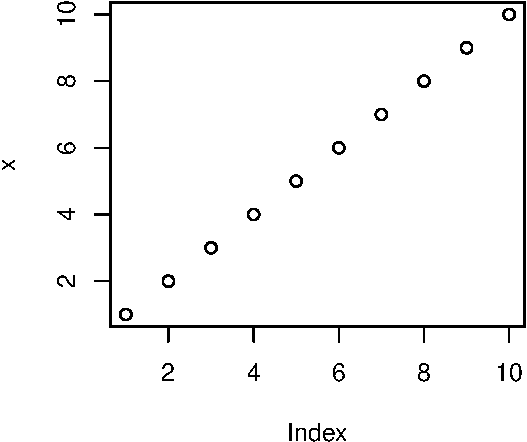
\includegraphics{paper_BiocF1000_files/figure-latex/plot-1.pdf}
\caption{\label{fig:plot}A caption to our sample plot.}
\end{figure}

\subsection{Tables}\label{tables}

Markdown syntax tends to lack some of the more sophisticated formatting
features available in LaTeX, so you may need to edit the tables later to
get the desired format.

\begin{table}[htbp]
\caption{Caption to table.}
\centering
\begin{tabledata}{@{}lll@{}}
\header First name & Last Name & Grade\\
\row John & Doe & 7.5\\
\row Richard & Miles & 2\\
\end{tabledata}
\end{table}

Just like figures, tables with captions will also be numbered and can be
referenced. Captions are entered as a paragraph beginning with the
string ``Table:'' (or just ``:''), which may appear either before or
after the table. A label for the table should appear in the beginning of
the caption in the form of \texttt{(\textbackslash{}\#tab:label)}, e.g.,
see Table \ref{tab:table}.

\begin{table}[htbp]
\caption{\label{tab:table} A table with text justification.}
\centering
\begin{tabledata}{@{}lcr@{}}
\header First name & Last Name & Grade\\
\row John & Doe & 7.5\\
\row Richard & Miles & 2\\
\end{tabledata}
\end{table}

\subsection{Figures}\label{figures}

You can include static figures (i.e.~no generated by code) using the
\texttt{include\_graphics()} function from the \textbf{knitr} package,
in a standard code chunk.

\begin{Shaded}
\begin{Highlighting}[]
\NormalTok{knitr}\OperatorTok{::}\KeywordTok{include_graphics}\NormalTok{(}\StringTok{'frog.jpg'}\NormalTok{)}
\end{Highlighting}
\end{Shaded}

\begin{figure}

{\centering 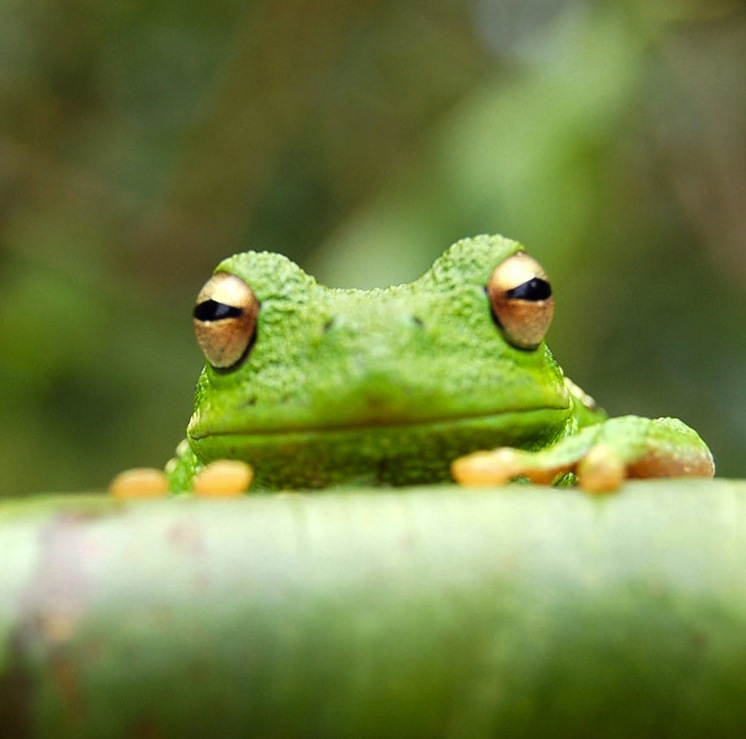
\includegraphics[width=0.5\linewidth]{frog} 

}

\caption{Your figure legend goes here; it should be succinct, while still explaining all symbols and abbreviations.}\label{fig:frog-picture}
\end{figure}

You can again use the \texttt{fig.cap} option to provide the figure
caption, and reference the image based on the code chunk label. You can
also use options such as \texttt{fig.align} and \texttt{fig.width} to
adjust the position and size of the image within the final document,
e.g.~Figure \ref{fig:frog-picture} is a frog.

Alternatively, you can use the standard markdown syntax like so:

\begin{figure}
\centering
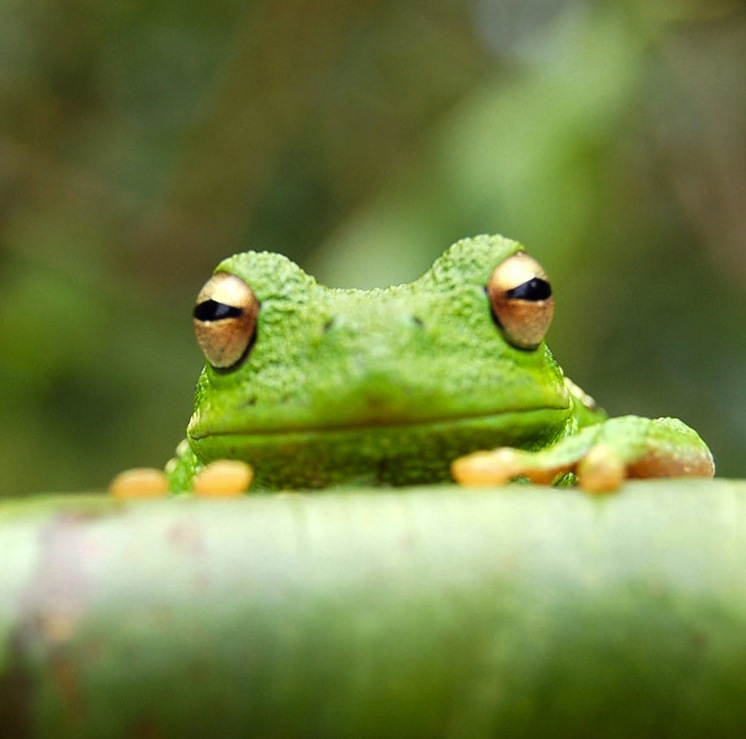
\includegraphics[width=0.25000\textwidth]{frog.jpg}
\caption{This is a smaller version of the same picture, inserted using
the standard markdown syntax}
\end{figure}

Please give figures appropriate filenames, e.g.: figure1.pdf,
figure2.png.

Figure legends should briefly describe the key messages of the figure
such that the figure can stand alone from the main text. However, all
figures should also be discussed in the article text. Each legend should
have a concise title of no more than 15 words. The legend itself should
be succinct, while still explaining all symbols and abbreviations. Avoid
lengthy descriptions of methods.

For any figures reproduced from another publication (as long as
appropriate permission has been obtained from the copyright holder
---see under the heading `Submission'), please include a line in the
legend to state that: `This figure has been reproduced with kind
permission from {[}include original publication citation{]}'.

\subsection{Mathematics}\label{mathematics}

You can use LaTeX syntax to typeset mathematical expressions. Let
\(X_1, X_2, \ldots, X_n\) be a sequence of independent and identically
distributed random variables with \(\text{E}[X_i] = \mu\) and
\(\text{Var}[X_i] = \sigma^2 < \infty\), and let
\[S_n = \frac{X_1 + X_2 + \cdots + X_n}{n}
      = \frac{1}{n}\sum_{i}^{n} X_i\] denote their mean. Then as \(n\)
approaches infinity, the random variables \(\sqrt{n}(S_n - \mu)\)
converge in distribution to a normal \(\mathcal{N}(0, \sigma^2)\).

To number and refer to equations, put them in the equation environments
and assign labels to them, as for Equation \eqref{eq:binom}.

\begin{equation}
  f\left(k\right) = \binom{n}{k} p^k\left(1-p\right)^{n-k}
  \label{eq:binom}
\end{equation}

\subsection{Lists}\label{lists}

You can make ordered lists

\begin{enumerate}
\def\labelenumi{\arabic{enumi}.}
\item
  Like this,
\item
  and like this.
\end{enumerate}

or bullet points

\begin{itemize}
\item
  Like this,
\item
  and like this.

  \begin{itemize}
  \item
    Use indentation

    \begin{itemize}
    \item
      for sub-items
    \end{itemize}
  \end{itemize}
\end{itemize}

DNA methylation is a fundamental epigenetic process known to play an
important role in controlling gene expression. It remains perhaps the
best studied biological mechanism amongst all known epigenetic processes
of its kind. With relatively recent advances in computational biology
and bioinformatics, probing DNA methylation has become rather easily
possible -- in fact, modern assays allow for DNA methylation signatures
at up to \(850,000\) CpG sites to be measured simultaneously. Most
statistical techniques available for the analysis of data produced by
such assays rely on (generalized) linear models. Here, we provide an
alternative to such approaches. Specifically, we provide a range of
\emph{variable importance measures} (\textbf{VIM}), parameters that
arise in statistical causal inference, for which targeted minimum
loss-based estimates may be readily computed based on the data made
available by DNA methylation assays. \texttt{methyvim} is an R package
that provides facilities for performing differential methylation
analyses within exactly this scope.

For a general discussion of the framework of targeted minimum loss-based
estimation and the role this approach plays in statistical causal
inference, the interested reader is invited to consult M. J. van der
Laan and Rose (2011) and M. J. van der Laan and Rose (2017). For a more
general introduction to (statistical) causal inference, Pearl (2009) and
Hernan and Robins (2018, forthcoming) may be of interest.

\begin{center}\rule{0.5\linewidth}{\linethickness}\end{center}

\subsection{Methodology}\label{methodology}

The core functionality of this package is made available via the
eponymous \texttt{methyvim} function, which implements a statistical
algorithm designed to compute targeted estimates of VIMs, defined in
such a way that the VIMs represent parameters of scientific interest in
computational biology experiments; moreover, these VIMs are defined such
that they may be estimated in a manner that is very nearly
assumption-free, that is, within a fully nonparametric statistical
model. \textbf{The statistical algorithm consists in several major
steps:}

\begin{enumerate}
\def\labelenumi{\arabic{enumi}.}
\item
  Pre-screening of genomic sites is used to isolate a subset of sites
  for which there is cursory evidence of differential methylation. For
  the sake of computational feasibility, targeted minimum loss-based
  estimates of VIMs are computed only for this subset of sites.
  Currently, the available screening approaches adapts core routines
  from the
  \href{http://bioconductor.org/packages/release/bioc/html/limma.html}{\texttt{limma}}
  R package, thought future releases will support functionality from
  other packages (e.g.,
  \href{https://CRAN.R-project.org/package=tmle.npvi}{\texttt{tmle.npvi}}).
\item
  Nonparametric estimates of VIMs (for the specified target parameter)
  are currently computed by adapting routines from the
  \href{https://CRAN.R-project.org/package=tmle}{\texttt{tmle}} R
  package. Future releases will support doubly-robust estimates of these
  VIMs (via the
  \href{https://cran.r-project.org/web/packages/drtmle/index.html}{\texttt{drtmle}}
  package) and add parameters for continuous treatments/exposures (via
  the
  \href{https://CRAN.R-project.org/package=tmle.npvi}{\texttt{tmle.npvi}}
  package).
\item
  Since pre-screening is performed prior to estimating VIMs, we make use
  of a multiple testing correction uniquely suited to such settings. Due
  to the multiple testing nature of the estimation problem, a variant of
  the Benjamini \& Hochberg procedure for controlling the False
  Discovery Rate (FDR) is applied (Benjamini and Hochberg 1995).
  Specifically, we apply the modified marginal Benjamini \& Hochberg
  step-up False Discovery Rate controlling procedure for multi-stage
  analyses (FDR-MSA), which is guaranteed to control the FDR as if all
  sites were tested (Tuglus and van der Laan 2009).
\end{enumerate}

\begin{center}\rule{0.5\linewidth}{\linethickness}\end{center}

\subsection{Parameters of Interest}\label{parameters-of-interest}

For discrete-valued treatments or exposures:

\begin{itemize}
\item
  The \emph{average treatment effect} (ATE): The effect of a binary
  exposure or treatment on the observed methylation at a target CpG site
  is estimated, controlling for the observed methylation at all other
  CpG sites in the same neighborhood as the target site, based on an
  additive form. In particular, the parameter estimate represents the
  \textbf{additive difference} in methylation that would have been
  observed at the target site had all observations received the
  treatment versus the scenario in which none received the treatment.
\item
  The \emph{relative risk} (RR): The effect of a binary exposure or
  treatment on the observed methylation at a target CpG site is
  estimated, controlling for the observed methylation at all other CpG
  sites in the same neighborhood as the target site, based on an
  geometric form. In particular, the parameter estimate represents the
  \textbf{multiplicative difference} in methylation that would have been
  observed at the target site had all observations received the
  treatment versus the scenario in which none received the treatment.
\end{itemize}

Support for continuous-valued treatments or exposures is \emph{planned
but not yet available}, though work is underway to incorporate into our
methodology the following

\begin{itemize}
\item
  A \emph{nonparametric variable importance measure} (NPVI) (Chambaz,
  Neuvial, and van der Laan 2012): The effect of continous-valued
  exposure or treatment (the observed methylation at a target CpG site)
  on an outcome of interest is estimated, controlling for the observed
  methylation at all other CpG sites in the same neighborhood as the
  target (treatment) site, based on a parameter that compares values of
  the treatment against a reference value taken to be the null. In
  particular, the implementation provided is designed to assess the
  effect of differential methylation at the target CpG site on a
  (typically) phenotype-level outcome of interest (e.g., survival), in
  effect providing an nonparametric evaluation of the impact of
  methylation at the target site on said outcome.
\end{itemize}

\emph{As previously noted, in all cases, an estimator of the target
parameter is constructed via targeted minimum loss-based estimation.}

Having now discussed the foundational principles of the estimation
procedure employed and the statistical algorithm implemented, it is best
to proceed by examining \texttt{methyvim} by example.

\begin{center}\rule{0.5\linewidth}{\linethickness}\end{center}

\subsection{Preliminaries: Setting up the
Data}\label{preliminaries-setting-up-the-data}

First, we'll load the \texttt{methyvim} package and the example data
contained in the \texttt{methyvimData} package that accompanies it:

\begin{Shaded}
\begin{Highlighting}[]
\KeywordTok{library}\NormalTok{(methyvim)}
\end{Highlighting}
\end{Shaded}

\begin{verbatim}
## methyvim: Nonparametric Differential Methylation Analysis with Variable Importance Measures
\end{verbatim}

\begin{verbatim}
## Version: 0.99.1
\end{verbatim}

\begin{Shaded}
\begin{Highlighting}[]
\KeywordTok{library}\NormalTok{(methyvimData)}
\end{Highlighting}
\end{Shaded}

Now, let's load the data set and seed the RNG:

\begin{Shaded}
\begin{Highlighting}[]
\KeywordTok{data}\NormalTok{(grsExample)}
\KeywordTok{set.seed}\NormalTok{(}\DecValTok{479253}\NormalTok{)}
\NormalTok{grsExample}
\end{Highlighting}
\end{Shaded}

\begin{verbatim}
## class: GenomicRatioSet 
## dim: 400 210 
## metadata(0):
## assays(2): Beta M
## rownames(400): cg23578515 cg06747907 ... cg01715842 cg09895959
## rowData names(0):
## colnames(210): V2 V3 ... V397 V398
## colData names(2): exp outcome
## Annotation
##   array: IlluminaHumanMethylationEPIC
## Preprocessing
##   Method: NA
##   minfi version: NA
##   Manifest version: NA
\end{verbatim}

The example data object is of class \texttt{GenomicRatioSet}, provided
by the \texttt{minfi} package. The summary provided by the
\texttt{print} method gives a wealth of information on the experiment
that generated the data -- since we are working with a simulated data
set, we need not concern ourselves with much of this information. While
most slots of objects of this S4 class have descriptive names, the
interested analyst might consider consulting the documentation of the
\texttt{minfi} package for an in-depth description (Aryee et al. 2014).

\begin{center}\rule{0.5\linewidth}{\linethickness}\end{center}

\subsection{Quantifying the Effect of an Exposure on DNA
Methylation}\label{quantifying-the-effect-of-an-exposure-on-dna-methylation}

\subsubsection{The Average Treatment Effect as Variable Importance
Measure}\label{the-average-treatment-effect-as-variable-importance-measure}

\ldots{}

\begin{Shaded}
\begin{Highlighting}[]
\KeywordTok{suppressMessages}\NormalTok{(}
\NormalTok{  methyvim_out_ate <-}\StringTok{ }\KeywordTok{methyvim}\NormalTok{(}\DataTypeTok{data_grs =}\NormalTok{ grsExample, }\DataTypeTok{sites_comp =} \DecValTok{10}\NormalTok{,}
                               \DataTypeTok{var_int =} \DecValTok{1}\NormalTok{, }\DataTypeTok{vim =} \StringTok{"ate"}\NormalTok{, }\DataTypeTok{type =} \StringTok{"Mval"}\NormalTok{,}
                               \DataTypeTok{filter =} \StringTok{"limma"}\NormalTok{, }\DataTypeTok{filter_cutoff =} \FloatTok{0.05}\NormalTok{,}
                               \DataTypeTok{parallel =} \OtherTok{FALSE}\NormalTok{, }\DataTypeTok{tmle_type =} \StringTok{"sl"}
\NormalTok{                              )}
\NormalTok{)}
\end{Highlighting}
\end{Shaded}

\begin{verbatim}
## Warning in set_parallel(parallel = parallel, future_param = future_param, : Sequential evaluation is strongly discouraged. 
##  Proceed with caution.
\end{verbatim}

\begin{Shaded}
\begin{Highlighting}[]
\NormalTok{methyvim_out_ate}
\end{Highlighting}
\end{Shaded}

\begin{verbatim}
## class: methytmle 
## dim: 400 210 
## metadata(0):
## assays(2): Beta M
## rownames(400): cg23578515 cg06747907 ... cg01715842 cg09895959
## rowData names(0):
## colnames(210): V2 V3 ... V397 V398
## colData names(2): exp outcome
## Annotation
##   array: IlluminaHumanMethylationEPIC
## Preprocessing
##   Method: NA
##   minfi version: NA
##   Manifest version: NA
\end{verbatim}

As is clear from examining the object \texttt{methyvim\_out\_ate}, the
output resembles exactly that returned when examining objects of class
\texttt{GenomicRatioSet} from the \texttt{minfi} R package. In
particular, the returned \texttt{methytmle} object is merely a modified
form (in particular, a subclass) of the input \texttt{GenomicRatioSet}
object -- thus, it contains all of the original slots, with all
experimental data intact. Several extra pieces of information are
contained within the output object as well\_.

We can take a look at the results produced from the estimation procedure
by examining the \texttt{"vim"} \texttt{slot} of the \texttt{methytmle}
object:

\begin{Shaded}
\begin{Highlighting}[]
\KeywordTok{head}\NormalTok{(}\KeywordTok{slot}\NormalTok{(methyvim_out_ate, }\StringTok{"vim"}\NormalTok{))}
\end{Highlighting}
\end{Shaded}

\begin{verbatim}
##            lowerCI_ATE     est_ATE upperCI_ATE    Var_ATE      pval
## cg22913481  -0.3790600 -0.10205080   0.1749584 0.01997451 0.4702524
## cg15131207  -0.3121142 -0.10416890   0.1037764 0.01125605 0.3261739
## cg10613282  -0.4272500 -0.16315679   0.1009364 0.01815525 0.2259382
## cg15857610  -0.3186500 -0.07896784   0.1607144 0.01495407 0.5184354
## cg24775884  -0.4696981  0.03989038   0.5494788 0.06759693 0.8780607
## cg22954484  -0.3289972  0.07614832   0.4812939 0.04272775 0.7125840
##            n_neighbors_all n_neighbors_w max_corr_w
## cg22913481               0             0         NA
## cg15131207               0             0         NA
## cg10613282               0             0         NA
## cg15857610               5             4  0.7720705
## cg24775884               5             2  0.8897566
## cg22954484               5             2  0.8643936
\end{verbatim}

From the table displayed, we note that we have access to point estimates
of the ATE (``est\_ATE'') as well as lower and upper confidence interval
bounds for each estimate (``lowerCI\_ATE'' and ``upperCI\_ATE'',
respectively). Additional statistical information we have access to
include the variance (``Var\_ATE'') of the estimate as well as the
p-value (``pval'') associated with each estimate (based on Wald-style
testing procedures). Beyond these, key bioinformatical quantities (with
respect to the algorithm outlined above) are also returned; these
include the total number of neighbors of the target site, the number of
neighboring sites controlled for when estimating the effect of exposure
on DNA methylation, and, finally, the maximum correlation between the
target site and any given site in its full set of neighbors.

\ldots{}

\begin{center}\rule{0.5\linewidth}{\linethickness}\end{center}

\subsubsection{The Risk Ratio as Variable Importance
Measure}\label{the-risk-ratio-as-variable-importance-measure}

\ldots{}

\begin{Shaded}
\begin{Highlighting}[]
\NormalTok{methyvim_out_rr <-}\StringTok{ }\KeywordTok{methyvim}\NormalTok{(}\DataTypeTok{data_grs =}\NormalTok{ grsExample, }\DataTypeTok{sites_comp =} \DecValTok{10}\NormalTok{,}
                            \DataTypeTok{var_int =} \DecValTok{1}\NormalTok{, }\DataTypeTok{vim =} \StringTok{"rr"}\NormalTok{, }\DataTypeTok{type =} \StringTok{"Mval"}\NormalTok{,}
                            \DataTypeTok{filter =} \StringTok{"limma"}\NormalTok{, }\DataTypeTok{filter_cutoff =} \FloatTok{0.05}\NormalTok{,}
                            \DataTypeTok{parallel =} \OtherTok{FALSE}\NormalTok{, }\DataTypeTok{tmle_type =} \StringTok{"sl"}
\NormalTok{                           )}
\end{Highlighting}
\end{Shaded}

\begin{verbatim}
## Warning in set_parallel(parallel = parallel, future_param = future_param, : Sequential evaluation is strongly discouraged. 
##  Proceed with caution.
\end{verbatim}

\begin{Shaded}
\begin{Highlighting}[]
\NormalTok{methyvim_out_rr}
\end{Highlighting}
\end{Shaded}

\begin{verbatim}
## class: methytmle 
## dim: 400 210 
## metadata(0):
## assays(2): Beta M
## rownames(400): cg23578515 cg06747907 ... cg01715842 cg09895959
## rowData names(0):
## colnames(210): V2 V3 ... V397 V398
## colData names(2): exp outcome
## Annotation
##   array: IlluminaHumanMethylationEPIC
## Preprocessing
##   Method: NA
##   minfi version: NA
##   Manifest version: NA
\end{verbatim}

\ldots{}

\begin{Shaded}
\begin{Highlighting}[]
\KeywordTok{head}\NormalTok{(}\KeywordTok{slot}\NormalTok{(methyvim_out_rr, }\StringTok{"vim"}\NormalTok{))}
\end{Highlighting}
\end{Shaded}

\begin{verbatim}
##            lowerCI_logRR    est_logRR upperCI_logRR    Var_logRR      pval
## cg22913481   -0.15978435 -0.042980967    0.07382242 0.0035513930 0.4707649
## cg15131207   -0.10832796 -0.036151215    0.03602553 0.0013560711 0.3262445
## cg10613282   -0.18349779 -0.069866731    0.04376433 0.0033611044 0.2281579
## cg15857610   -0.07196023 -0.018317791    0.03532465 0.0007490399 0.5033043
## cg24775884   -0.07914787  0.006261306    0.09167049 0.0018988776 0.8857479
## cg22954484   -0.06728830  0.015365555    0.09801941 0.0017783369 0.7155826
##            n_neighbors_all n_neighbors_w max_corr_w
## cg22913481               0             0         NA
## cg15131207               0             0         NA
## cg10613282               0             0         NA
## cg15857610               5             4  0.7720705
## cg24775884               5             2  0.8897566
## cg22954484               5             2  0.8643936
\end{verbatim}

\ldots{}

\begin{center}\rule{0.5\linewidth}{\linethickness}\end{center}

\subsection{Visualization of Results}\label{visualization-of-results}

\ldots{}

\begin{Shaded}
\begin{Highlighting}[]
\KeywordTok{plot}\NormalTok{(methyvim_out_rr, }\DataTypeTok{type =} \StringTok{"volcano"}\NormalTok{)}
\end{Highlighting}
\end{Shaded}

\ldots{}

\begin{Shaded}
\begin{Highlighting}[]
\KeywordTok{plot}\NormalTok{(methyvim_out_rr, }\DataTypeTok{type =} \StringTok{"pvals"}\NormalTok{)}
\end{Highlighting}
\end{Shaded}

\ldots{}

\begin{Shaded}
\begin{Highlighting}[]
\KeywordTok{plot}\NormalTok{(methyvim_out_rr, }\DataTypeTok{type =} \StringTok{"heatmap"}\NormalTok{)}
\end{Highlighting}
\end{Shaded}

\ldots{}

\begin{center}\rule{0.5\linewidth}{\linethickness}\end{center}

\subsection*{References}\label{references}
\addcontentsline{toc}{subsection}{References}

\hypertarget{refs}{}
\hypertarget{ref-aryee2014minfi}{}
Aryee, Martin J, Andrew E Jaffe, Hector Corrada-Bravo, Christine
Ladd-Acosta, Andrew P Feinberg, Kasper D Hansen, and Rafael A Irizarry.
2014. ``Minfi: A Flexible and Comprehensive Bioconductor Package for the
Analysis of Infinium DNA Methylation Microarrays.''
\emph{Bioinformatics} 30 (10). Oxford University Press (OUP): 1363--9.
doi:\href{https://doi.org/10.1093/bioinformatics/btu049}{10.1093/bioinformatics/btu049}.

\hypertarget{ref-benjamini1995controlling}{}
Benjamini, Yoav, and Yosef Hochberg. 1995. ``Controlling the False
Discovery Rate: A Practical and Powerful Approach to Multiple Testing.''
\emph{Journal of the Royal Statistical Society. Series B
(Methodological)}. JSTOR, 289--300.

\hypertarget{ref-chambaz2012estimation}{}
Chambaz, Antoine, Pierre Neuvial, and Mark J van der Laan. 2012.
``Estimation of a Non-Parametric Variable Importance Measure of a
Continuous Exposure.'' \emph{Electronic Journal of Statistics} 6. NIH
Public Access: 1059.

\hypertarget{ref-hernan2018causal}{}
Hernan, Miguel A, and James M Robins. 2018, forthcoming. \emph{Causal
Inference}. Chapman \& Hall/Crc Texts in Statistical Science. Taylor \&
Francis.

\hypertarget{ref-Smith:2013jd}{}
Jones, A. B., and J. M. Smith. 2013. ``Article Title.'' \emph{Journal
Title} 13 (52). Publisher: 123--456.

\hypertarget{ref-pearl2009causality}{}
Pearl, Judea. 2009. \emph{Causality: Models, Reasoning, and Inference}.
Cambridge University Press.

\hypertarget{ref-Smith:2012qr}{}
Smith, J. M., and A. B. Jones. 2012. \emph{Book Title}. 7th ed.
Publisher.

\hypertarget{ref-tuglus2009modified}{}
Tuglus, Catherine, and Mark J. van der Laan. 2009. ``Modified FDR
Controlling Procedure for Multi-Stage Analyses.'' \emph{Statistical
Applications in Genetics and Molecular Biology} 8 (1). Walter de
Gruyter: 1--15.
doi:\href{https://doi.org/10.2202/1544-6115.1397}{10.2202/1544-6115.1397}.

\hypertarget{ref-vdl2011targeted}{}
van der Laan, Mark J, and Sherri Rose. 2011. \emph{Targeted Learning:
Causal Inference for Observational and Experimental Data}. Springer
Science \& Business Media.

\hypertarget{ref-vdl2017targeted}{}
---------. 2017. \emph{Targeted Learning in Data Science: Causal
Inference for Complex Longitudinal Studies}. Springer Science \&
Business Media.

\end{document}
